%!TEX root = ../main.tex
% !TeX spellcheck = en_GB 
% Chapter 2
%------------------------------------------------------------------------------------
\chapter{Theory} % Main chapter title

\label{Theory} % For referencing the chapter elsewhere, use \ref{Chapter1}
%------------------------------------------------------------------------------------
\section{Unmanned Surface Vehicles}
\cite{jokioinen2016remote}

Unmanned Surface Vehicles (USV) or Autonomous Surface Crafts (ASC) are vehicles operating the seas without a crew on-board.
USVs encompass both fully autonomous vehicles, from now on referred to as ASCs, and semi-autonomous vehicles.
Development of USVs has been ongoing for the last two decades \cite{manley2008unmanned}.
However, majority of the USVs developed are of the semi-autonomous type \cite{liu2016unmanned,park2017development}, meaning that they depend on human intervention to some extent usually by a supervisor located on shore.
Although semi-autonomous USVs greatly increase the safety of the operating personnel \cite{liu2016unmanned}, they do not completely remove the need for human interaction.
Supervision of several semi-autonomous vehicles can be admittedly be handled by a single person, which significantly decreases the amount of person-hours needed to accomplish a specific mission \cite{manley2008unmanned}.
The person-hours needed for surveillance could, however, be removed completely by a ASC.
It is, therefore, of great interest to overcome the challenges associated with ASCs.


%------------------------------------------------------------------------------------
\subsection{Usage}
\textcite{Yuh2011} mention that roughly two-thirds of the earth's surface is covered by water, with an average depth of the oceans being 3688 m \cite{depth_ocean}.
Thereby, adding up to vast amount of explorable areas of which 95 \% is yet to be seen by human eyes \cite{explored_percentage}.
Although ASCs are situated on the surface of the ocean they can greatly increase the efficiency of Unmanned Underwater Vehicles (UUV) by acting as a gateway between UUVs and services, such as GPS, not easily available in underwater environments \cite{liu2016unmanned}.


\textcite{liu2016unmanned} have, furthermore, compiled a list of potential applications of USVs, along with previous research on the topics.
The list is divided into four major categories: Scientific research, Environmental missions, Ocean resource exploration and Other applications.
Many of the applications mentioned would require the vehicles to interact with other vessels.
It is therefore crucial for the USVs to follow the Convention on the International Regulations for Preventing Collisions at Sea, 1972 (COLREGs) explained in section \ref{sec_colreg}.


%\subsection{Current state}
%------------------------------------------------------------------------------------
\subsection{Challenges}
limited autonomy due to the challenges in automated and reliable guidance, navigation and control (GNC) functions for all different operating conditions in face of sophisticated and hazardous environments, and sensor, actuator and communication failures \cite{liu2016unmanned}.
%------------------------------------------------------------------------------------
\section{COLREG}
\label{sec_colreg}
Convention on the International Regulations for Preventing Collisions at Sea, 1972 (COLREGs) consist of 38 rules, grouped into five different sections, designed by the International Maritime Organization (IMO).
The rules were adopted 1972 and entered into force 1977.
COLREGs was designed to ensure traffic separation between vessels in an increasingly populated environment back in 1972, and it is, therefore, sometimes referred to as the Rules of the Road for maritime vessels.
COLREGs has since been in use and mandatory to adhere to on international waters, although it has received amended several times \cite{colreg_about_imo}.

National regulations might differ from the COLREGs to some extent. However, COLREG mention that ‘Nothing in these Rules shall interfere with the operation of special rules made by an appropriate authority for
roadsteads, harbours, rivers, lakes or inland waterways connected with the high seas and navigable by seagoing
vessels.
Such special rules shall conform as closely as possible to these Rules.’ \cite{colreg}

%------------------------------------------------------------------------------------
\subsection{Parts}
This subsection will present the different parts of the COLREGs regulations, with emphasis on the parts related to manoeuvring an USV in international waters. Information in this subsection is taken from the official COLREG regulations  \cite{colreg} if not otherwise specified.
%------------------------------------------------------------------------------------
\subsubsection{Part A General}
\textbf{Rule 1} cover which vessels that are affected by the COLREGs regulations. This includes all vessels navigation on high seas and all waters connected therewith.
Additionally, it specifies that special rules regarding roadsteads, harbours, rivers, lakes or inland waterways connected with the high seas and navigable by seagoing, shall conform as closely as possible to these Rules.
\\
\textbf{Rule 2} states that the COLREG rules does not in any way free the vessel, owner, master or crew from responsibility to follow the rules and act according to ordinary practice of seamen.
\\
\textbf{Rule 3} Defines the meaning of words used in the regulations, such as: vessel, power-driven vessel, sailing vessel, length, and breadth.
%------------------------------------------------------------------------------------
\subsubsection{Part B Steering and Sailing}
\textbf{Rule 4} simply states that all rsimply states that all Rules in Part B Section I (rules 4-10) apply in any condition of visibilitysimply states that all Rules in Part B Section I (rules 4-10) apply in any condition of visibilityules in Part B Section I (rules 4-10) apply in any condition of visibility
\\
\textbf{Rule 5} states that all vessels shall at all times maintain proper look-out by sight and hearing and all other available means to ensure the best possible situation awareness.
\\
\textbf{Rule 6} states that vessels shall maintain a speed so that they can take proper and effective action to avoid collision and stop within distance appropriate to the prevailing circumstances and conditions.
\\
\textbf{Rule 7} state that all vessels shall use all means possible to determine if there is a risk of collision.
This includes the use of radar equipment, however, caution should be exercised not to trust insufficient data.
Moreover, Rule 7 states that any doubt whether a risk of collision exists, shall be treated as if a risk exists.
Finally it specifies that a constant compass bearing between two vessels, means that the two vessels are on collision course with each other.
However, a constant bearing is only a sufficient condition for a risk of collision not a necessary one.
Close range, large vessels or a tow might pose a collision risk, without a constant bearing.
\\
\textbf{Rule 8} concerns actions to avoid collision. Actions shall, for instance, taken according to the rules and as far as possible be conducted in ample time and large enough so that they are easily observable by other vessels. Small alterations should in other words be avoided. Course alterations might, moreover, be accompanied by a lowering of speed, if necessary to ensure in the vessels passing each other at safe distance.
\\
\textbf{Rule 9} concerns navigation in narrow channels and is therefore not of interest for the scope of this thesis.
\\
\textbf{Rule 10} Concerns Traffic Separation Schemes ruled by IMO. These are traffic route systems developed for particularly congested shipping areas \cite{ships_routing_imo} and, therefore, not of interest for the scope of this thesis.
\\
\textbf{Rule 11} simply states that all rules in Part B Section II (rules 11-18) apply to vessels in sight of each other.
\\
\textbf{Rule 12} concerns sailing vessels and is therefore not of interest for the scope of this thesis.
\\
\textbf{Rule 13} specifies action to be taken by a vessel (give way vessel) when overtaking another vessel (stand on vessel). The give way vessel shall keep out of the way of the stand on vessel. A vessel is considered to overtake another vessel when approaching the other stand on vessel from a direction more than 22.5 \textdegree abaft the stand on vessels beam, i.e with a relative bearing between 112,5 \textdegree and 247,5 \textdegree from the stand on vessel.
\\
\textbf{Rule 14} defines a head-on situation as well as actions to be taken in case of a head-on situation. A head-on situation is when a vessel sees another vessel ahead or nearly ahead, i.e. it can see the masthead light in line or both sidelights. The give way vessel shall in this case alter its course to starboard.
\\
\textbf{Rule 15} states that vessel coming from starboard, i.e right, has the right of way in a crossing situation. The give way vessel shall if possible avoid crossing ahead of the other vessel and, therefore, alter its course to starboard.
\\
\textbf{Rule 16} states that give way vessel shall take action as early as possible.
\\
\textbf{Rule 17} states that give way vessels shall keep their course and speed, provided that the give way vessel acts according to the regulations or if the actions by the give way vessels are insufficient to prevent a collision.
\\
\textbf{Rule 18} specifies responsibilities between vessels of different type. For instance a power driven vessel shall give way for a vessel engaged in fishing.
\\
\textbf{Rule 19} specifies reduced visibility operations. Vessels should proceed at speeds appropriate to the circumstances and use radar to determine collision risks. Speed should be reduced to minimum if a vessel can hear another vessels fog horn apparently forward of her beam.

%------------------------------------------------------------------------------------
\subsubsection{Part C Lights and Shapes}
Part C specifies the lights and shapes a vessel shall exhibit, and when they should be used. These are therefore not of interest for the scope of this thesis, with the exception of \textit{rule 21 and 22}, which specify the arcs that specific lights should cover as well as the distance the should be visible from.
\\
\textbf{Masthead lights} cover a 225 \textdegree arc from 247,5 \textdegree to 112,5 \textdegree and should be visible from at least 2-6 miles, depending on the length of the vessel.\\
\textbf{Sidelights} are green on starboard side and red on port. They cover a 112,5 arc from 0 relative bearing to 112,5 and 247,5 respectively. They should be visible from at least 1-3 miles, depending on the length of the vessel.
%------------------------------------------------------------------------------------
\subsubsection{Part D Sound and Light signals}
Part D specifies sound and light signals and is not of interest for the scope of this thesis.
%------------------------------------------------------------------------------------
\subsubsection{Part E Exemptions}
Is not of interest for the scope of this thesis.


%------------------------------------------------------------------------------------

\section{Previous research Collision Avoidance Algorithms}
Compiled from from \cite{liu2016unmanned}
Protocol-free collision avoidance:

%------------------------------------------------------------------------------------
\subsection{obstacles are assumed to be enclosed by elliptical shapes, differential equations } \cite{soltan2009trajectory}
\begin{itemize}
    \con obstacles approximated as elliptic shapes
    \con Focuses mostly on under-actuated unmanned surface vessels
    \con Does not mention COLREG
    \pro  only the current information about the obstacles and the target are required for real-time trajectory planning
    \item ellipses represent stable limit cycle solution
    \item planned trajectories are tracked by the vessel through a sliding mode control law which is robust to environmental  disturbances  and  modeling uncertainties and can be computed in real time
\end{itemize}
%------------------------------------------------------------------------------------
\subsection{path re-planning approach based on the level set methods }\cite{xu2013fast}
\begin{itemize}
    \con environment is static
    \con method can be slow for very large areas
\end{itemize}
%------------------------------------------------------------------------------------
\subsection{angular rate-constrained  Theta* ( ARC - Theta* )  }\cite{kim2014angular}
\begin{itemize}
    \con Does not consider colreg atm (future work)
    \pro  considering both angular rate (yaw rate) and heading angle of unmanned surface vehicles (USVs)
    \item Based on Theta*
    \item  proposed to create paths in real-time with considerations of vehicle performance on the SE(2) weighted occupancy grid map
\end{itemize}
%------------------------------------------------------------------------------------
\subsection{optical-flow based approach }\cite{el2013visual}
\begin{itemize}
    \pro low computational cost
    \con made for low cost low-cost autonomous watercraft in riverine environments, such as lakes and rivers
    \con uses only a mobile phone
    \con assuming that the water surface consists of a horizontal plane
    \con static objects
\end{itemize}
%------------------------------------------------------------------------------------
\subsection{lattice-based path planning method }\cite{bertaska2013experimental}
\begin{itemize}
    \con Can not find a free copy
\end{itemize}
%------------------------------------------------------------------------------------
\subsection{underwater collision avoidance}\cite{heidarsson2011obstacle,onunka2013probabilistic}

%------------------------------------------------------------------------------------
\subsection{direct method based on inverse dynamics in the virtual domain (IDVD) }\cite{yakimenko2011real}


Protocol-based collision avoidance:
\subsection{modified virtual force field (MVFF) }\cite{lee2004fuzzy}

%------------------------------------------------------------------------------------
\subsection{behavior-based control and multi-objective action selection} \cite{benjamin2004colregs,benjamin2006method}

%------------------------------------------------------------------------------------
\subsection{near-field reactive control technique }\cite{larson2007advances}

%------------------------------------------------------------------------------------
\subsection{relative coordinate based collision avoidance strategy with integration of an evolutionary path planner }\cite{zhuang2011motion}

%------------------------------------------------------------------------------------
\subsection{simple manual biasing scheme and a direction priority sequential selection (DPSS) strategy under COLREGs. }\cite{naeem2012colregs}
%------------------------------------------------------------------------------------
\subsection{ a rule-based repairing A* ( R - RA* ) algorithm in com-
    pliance with COLREGs }\cite{campbell2014automatic}

%------------------------------------------------------------------------------------
\subsection{velocity obstacles (VO) }\cite{kuwata2014safe}

%------------------------------------------------------------------------------------
\subsection{Trajectory planning with adaptive control primitives
    for autonomous surface vehicles operating in congested civilian traffic }\cite{shah2014trajectory}

%------------------------------------------------------------------------------------
\subsection{other } \cite{svec2013dynamics,vsvec2016adaptive,svec2012automated,svec2012usv}

%------------------------------------------------------------------------------------
\section{Fuzzy set theory and logic}
The concept of fuzzy sets was first mentioned by \textcite{zadeh1996fuzzy} in 1964 as a way of dealing with sets of objects, where an objects membership to a set can be represented by a value in the real interval [0, 1]. Compared to classic set theory where to membership is restricted to the two values of one and zero. Fuzzy logic enables one to define sets such as "old men" or "vessels on nearly reciprocal course" \cite{zadeh1996fuzzy}, which facilitates the process of converting human abstract reasoning into computer understandable logic.
%------------------------------------------------------------------------------------
\subsection{Fuzzy sets}
The fuzzy set "all old men" can be defined in the following way. Let the \textit{universe set} \textbf{X} be the set of ages [0, 100]. The set of old men can then be written as
$\fuzzyset{A}=\left \{ a \in \textbf{X} | a \text{ is old} \right \}$
\cite{chen2000introduction}

However, the set requirement 'is old' is still undefined and therefore vague. Defining the threshold of being old at an age of 60 does divide the universal set \textbf{X} into subsets of 'old' and 'not old', but the division does not distinguish between humans aged 1 and 59.
Fuzzy set theory introduces the concept of membership functions, to solve this problem. A Fuzzy Membership Function (FMF) describes the grade of membership of a  in  $\fuzzyset{A}$. This function is often written as $\mu_{\fuzzyset{A}}(a)$. Figure \ref{fig:FMF_ex} shows a very simple linear FMF for the example $\fuzzyset{A}=\left \{\text{'is old'} \right \}$, where for instance $\mu_{\fuzzyset{A}}(10)=0.1$. Similar FMFs can be defined for young and middle-aged which results in the graph seen in figure \ref{fig:FMF_ex2} \cite{ross2009fuzzy}.

A fuzzy set can then be written as an array of tuples consisting of the objects and its associated membership value: $\fuzzyset{A}=\left \{(x,\mu_{\fuzzyset{A}}(x)|x \in X) \right \}$ \cite{zimmermann2010fuzzy}, which gives \\ $\fuzzyset{A}=\left \{(0,1),(10,0.9),(20,0.8),\dots,(90,0.1),(100,0) \right \}$ for the example $\fuzzyset{A}$=\{'is young'\} in figure \ref{fig:FMF_ex} \cite{ross2009fuzzy}.
\begin{figure}
    \centering
    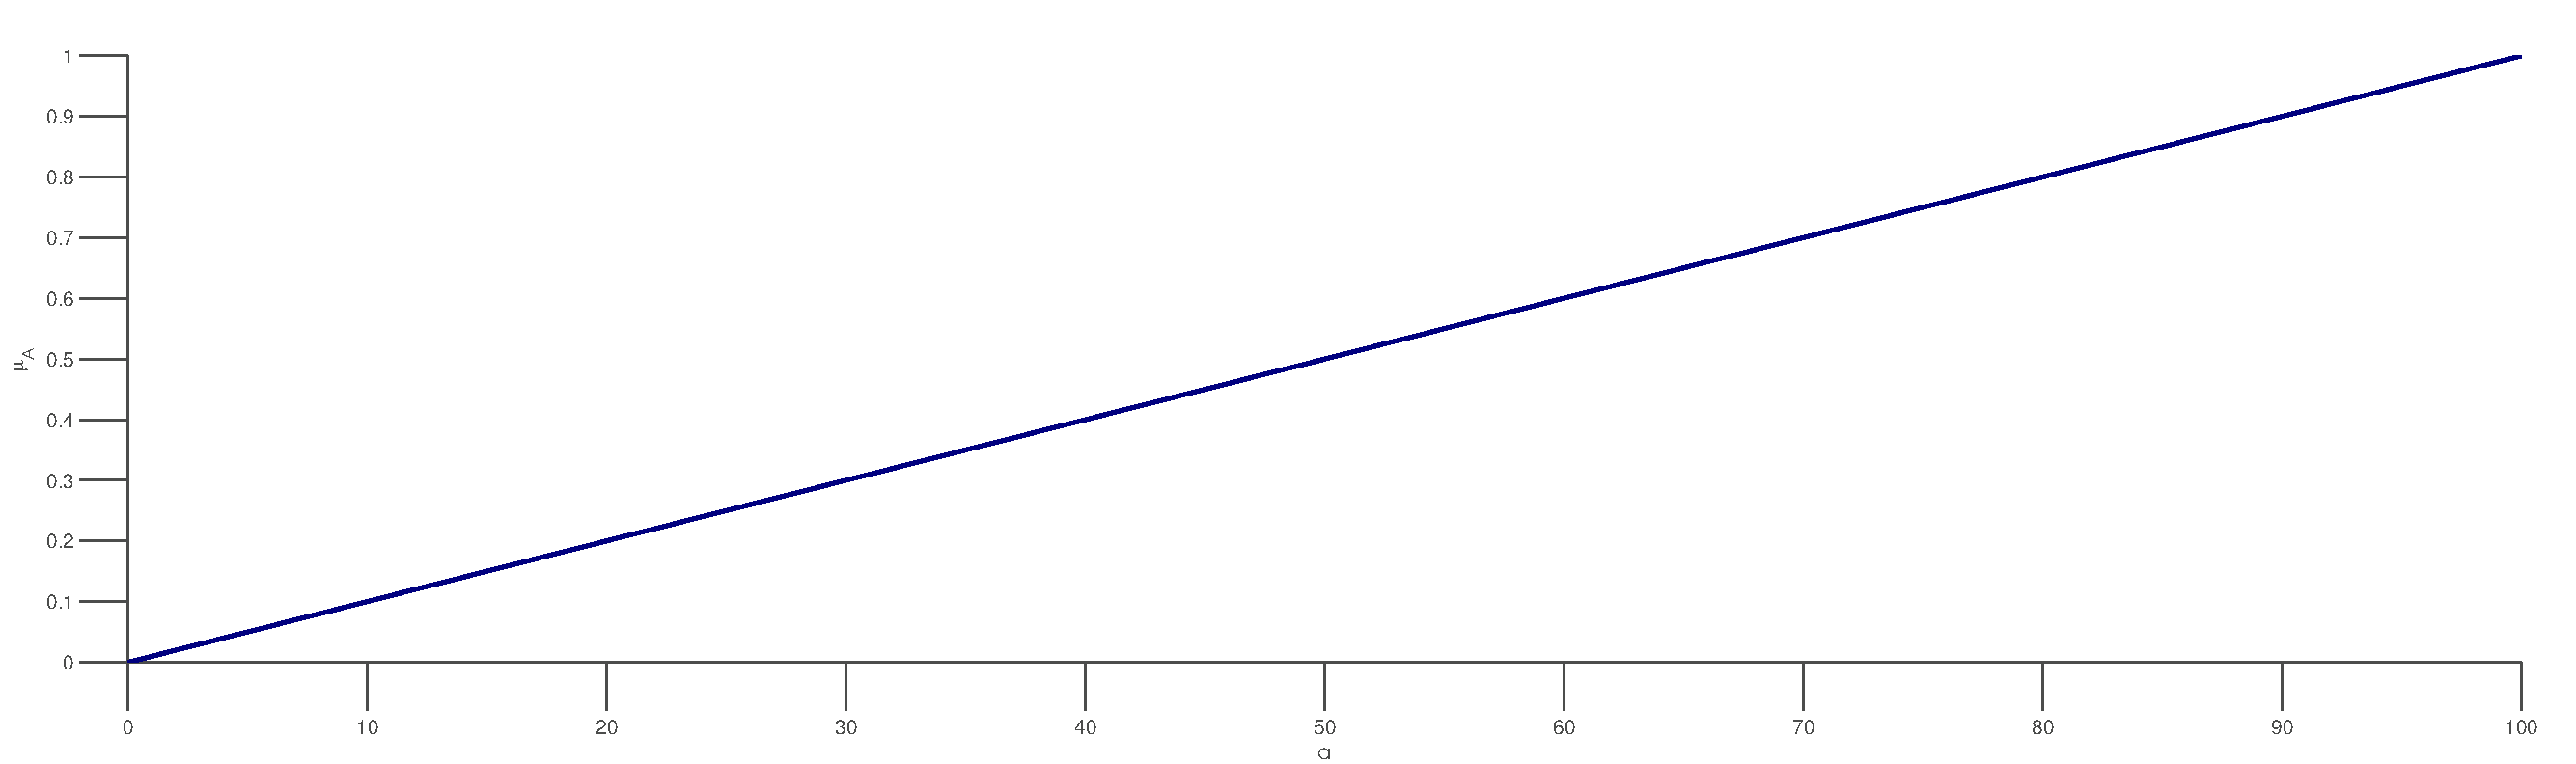
\includegraphics[width=\textwidth]{FMF_ex}
    \caption{Fuzzy membership function for $\protect\fuzzyset{A}=\left \{ \text{'Is old'} \right \}$}
    \label{fig:FMF_ex}
\end{figure}

\begin{figure}
    \centering
    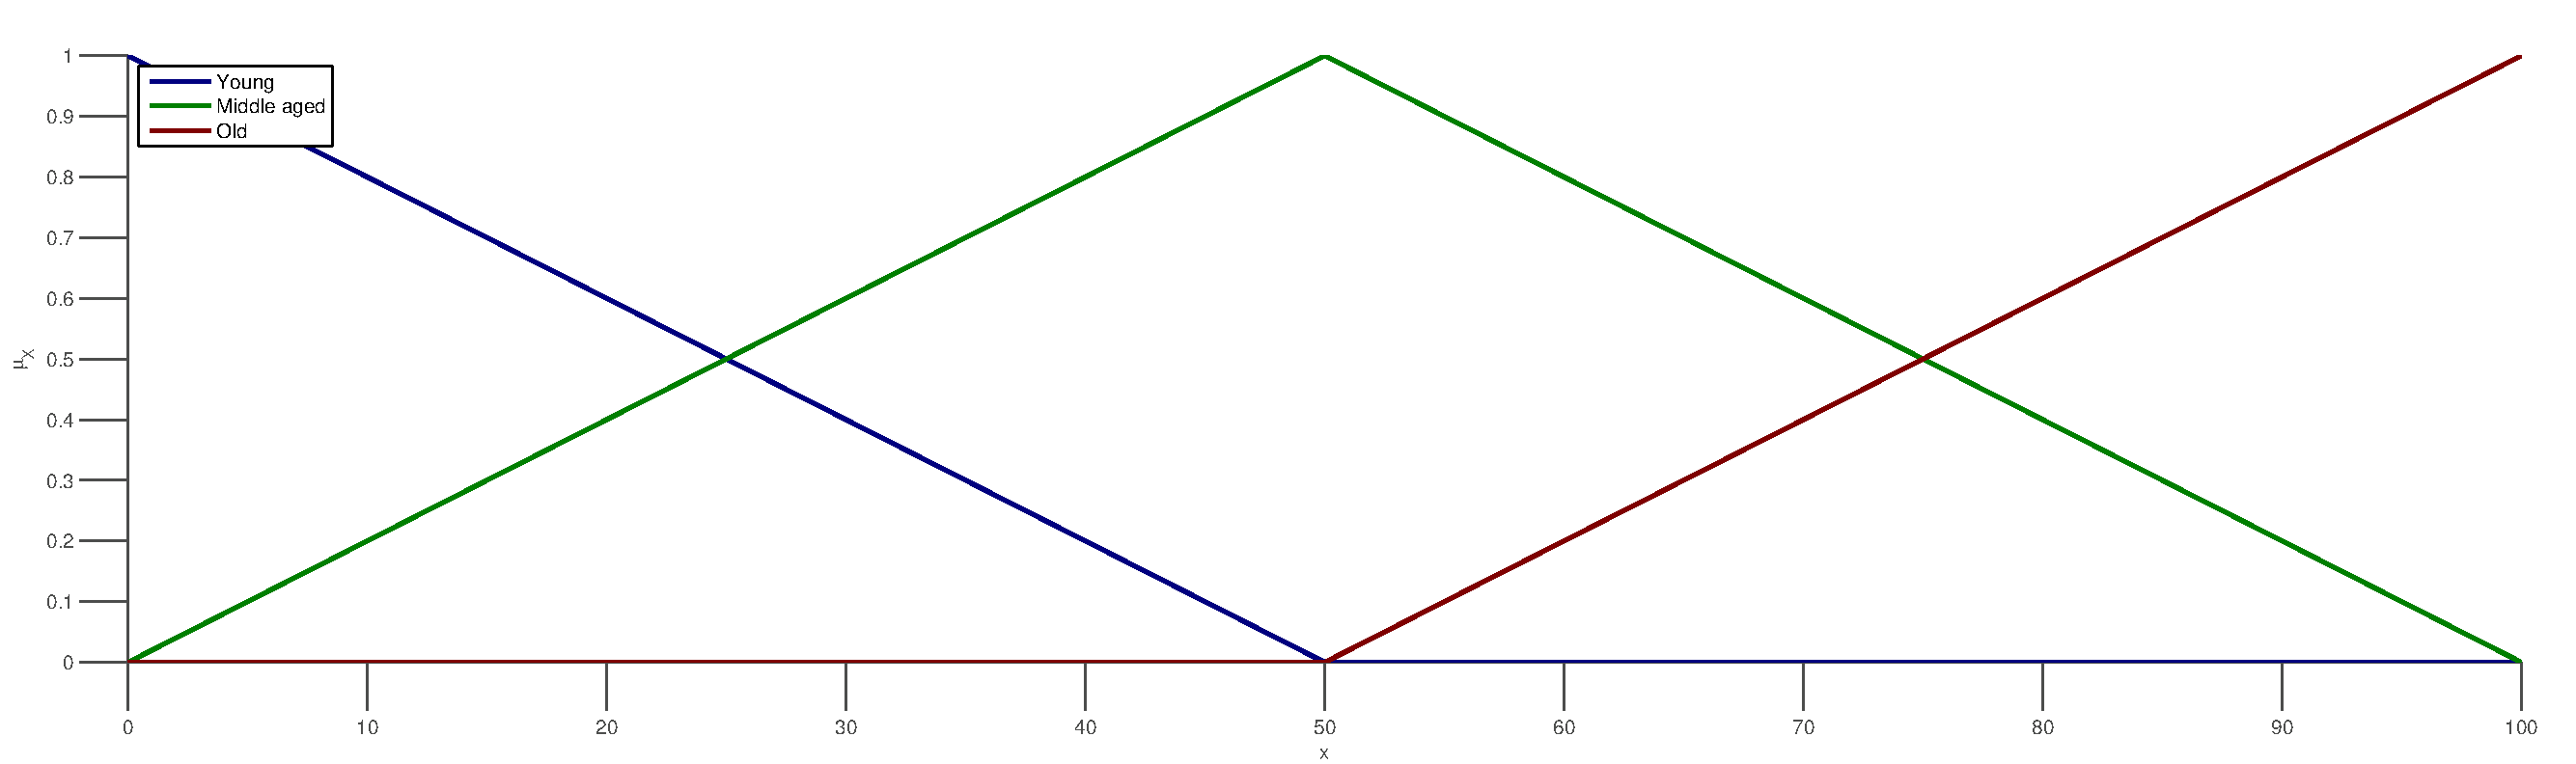
\includegraphics[width=\textwidth]{FMF_ex2}
    \caption{Fuzzy membership function for $\protect\fuzzyset{A}=\{\text{'Is young'}\}, \protect\fuzzyset{B}=\{\text{'Is middle-aged'\}}\text{ and }\protect\fuzzyset{C}=\{\text{'Is old'}\}$}
    \label{fig:FMF_ex2}
\end{figure}
%------------------------------------------------------------------------------------
\subsection{Fuzzy logic}
Fuzzy sets and set theory can in the same manner as classical boolean sets be used to define logical expressions. Fuzzy logic allows for half-truths, i.e. truth values in the interval [0,1]. Whereas boolean logic is restricted to truth values of one and zero. The truth value T of a fuzzy preposition P is, therefore a mapping from [0,1] to the universe T, as can be seen in \ref{eq:fuzzy-logic-mapping} \cite{ross2009fuzzy}.
\begin{equation}
    T:u\in U\rightarrow (0,1)
    \label{eq:fuzzy-logic-mapping}
\end{equation}
The truth value of proposition P $(T(P))$ is therefore given by the membership grade $\mu_{\fuzzyset{A}}(x)$ of $x$ in $\fuzzyset{A}$

Many of the same operators and connectives used in classical logic, does also apply to fuzzy logic. This thesis will only present the rules necessary for the scope of the thesis, which are the following \cite{ross2009fuzzy}:\\
\noindent Negation
\begin{equation}
    T(\fuzzyset{\overline{P}})=1-T(\fuzzyset{P})) {}\label{eq:negation}
\end{equation}
Disjunction
\begin{equation}
    \fuzzyset{P}\lor \fuzzyset{Q}:x \text{ is } \fuzzyset{A} \text{ or } \fuzzyset{B}\quad T(\fuzzyset{P} \lor \fuzzyset{Q})=max(T(\fuzzyset{P}),T(\fuzzyset{Q}))\label{eq:disjunction}
\end{equation}
Conjunction
\begin{equation}
    \fuzzyset{P}\land \fuzzyset{Q}:x \text{ is } \fuzzyset{A} \text{ or } \fuzzyset{B}\quad T(\fuzzyset{P} \land \fuzzyset{Q})=min(T(\fuzzyset{P}),T(\fuzzyset{Q}))\label{eq:conjunction}
\end{equation}
Implication
\begin{equation}
    \fuzzyset{P}\to \fuzzyset{Q}: x \text{ is } \fuzzyset{A} \text{, then }x \text{ is } \fuzzyset{B}
    \label{eq:implication}
\end{equation}
\[ T(\fuzzyset{P}\to \fuzzyset{Q})=T(\fuzzyset{\overline{P}}\lor\fuzzyset{Q})=max(T(\fuzzyset{\overline{P}}),T(\fuzzyset{Q}))  \]

\noindent Implication can also be written in rule based form
\[ \fuzzyset{P} \to \fuzzyset{Q} \text{ is  IF } x \text{ is } \fuzzyset{A} \text{ , THEN } t \text{ is } \fuzzyset{B}\]
\[ \Leftrightarrow \]
\[  R=(\fuzzyset{A}\times\fuzzyset{B})\cup (\overline{\fuzzyset{A}}\times \fuzzyset{Y})\]
\noindent With the membership function:
\begin{equation}
    \mu_{\fuzzyset{R}}(x,y)=max[\mu_{\fuzzyset{A}}(x)\land\mu_{\fuzzyset{B}}(y),(1-\mu_{\fuzzyset{A}}(x))]
    \label{eq:implication-orig}
\end{equation}
Equation \ref{eq:implication-orig} is equivalent to the material implication used in traditional boolean logic \cite{ying2002implication}. However, fuzzy logic has multiple implication operators \cite{ross2009fuzzy}. The work in this thesis will use Mamdani's impication , see equation \ref{eq:mamdani}.
\begin{equation}
    \mu_{\fuzzyset{R}}(x,y)=min[\mu_{\fuzzyset{A}}(x),\mu_{\fuzzyset{B}}(x))]
    \label{eq:mamdani}
\end{equation}




%------------------------------------------------------------------------------------
\subsection{Fuzzy (rule-based) systems}
Fuzzy logic can be used to model complex systems described in natural language, originally written to be interpreted by humans. Such knowledge can often be written as rules in the following form \cite{ross2009fuzzy}.
\begin{equation}
    \text{IF premise (antecedent), THEN conclusion (consequent)}
\end{equation}
Combining multiple rules enables one to describe complex systems in a relatively simple structure. Rules can, furthermore, contain multiple antecedents and consequents. However, this raises the question of how multiple antecedents, as shown in rule \ref{eq:conj-ant}, can be  decomposed into a single antecedent and the rules aggregated into a single consequent \cite{ross2009fuzzy}.
\begin{equation}
    \text {IF $x$ is $\fuzzyset{A_1}$ and $\fuzzyset{A_2}$ \dots and $\fuzzyset{A_L}$ THEN $y$ is $\fuzzyset{B_s}$}
    \label{eq:conj-ant}
\end{equation}
Conjunctive antecedents can rewritten as a new fuzzy set

\[ \fuzzyset{A_s}=\fuzzyset{A_1}\cap \fuzzyset{A_2} \cap \dots \cap \fuzzyset{A_L} \]
with the membership function
\[ \mu_{\fuzzyset{A_S}}(x)=min \left [\mu_{\fuzzyset{A_1}}(x),\mu_{\fuzzyset{A_2}}(x),\dots,\mu_{\fuzzyset{A_3}}(x) \right ] \]
Rule \ref{eq:conj-ant} can then be rewritten as
\[ \text{IF $\fuzzyset{A_S}$ THEN $\fuzzyset{B_S}$} \]
Disjunctive antecedents can similarly be written as
\[ \fuzzyset{A_s}=\fuzzyset{A_1}\cup \fuzzyset{A_2} \cup \dots \cup \fuzzyset{A_L} \]
\[ \mu_{\fuzzyset{A_S}}(x)=max \left [\mu_{\fuzzyset{A_1}}(x),\mu_{\fuzzyset{A_2}}(x),\dots,\mu_{\fuzzyset{A_3}}(x) \right ] \]
The same principle can be applied to find the overall consequent when multiple rules apply. Conjunctive rules where both consequents must be applied, can be found by  the fuzzy intersection of all the rule consequents. Whereas disjunctive rules use the fuzzy union of the rule consequents.

%\subsection{Global path planning}
%\subsection{Protocol-based collision avoidance}
%\subsection{Protocol-free collision avoidance}
%\subsection{State estimation}
%\section{Spatial–temporal reasoning}
